\documentclass[../Main.tex]{subfiles}

\begin{document}
\chapter{Wahrscheinlichkeit und Statistik}

\intro{

}

\section{Kombinatorik}
Die Kombinatorik ist eine Teildisziplin der Mathematik, die sich mit endlichen oder abzählbar unendlichen diskreten Strukturen beschäftigt und deshalb auch dem Oberbegriff Diskrete Mathematik zugerechnet wird.
\defn{Produktregel (Für-jede-gibt-es-Regel)}{
Wenn es für jede von \(n\)  Wahlmöglichkeiten m mögliche weitere Wahlmöglichkeiten gibt, dann gibt es insgemsamt \(n \cdot m\)  Möglichkeiten. 
\begin{equation}
    n_1 \cdot n_2 \dots n_k = \prod_{i=1}^k n_i
\end{equation}
}

\defn{Permutation (Anordnung)}{
Gegeben sind \(n\)  anzuordnende Objekte. Die Fakultät ! beschreibt dabei die Anzahl Arten wie dies geschehen kann.
\begin{equation}
    \begin{split}
        P_n &= \#\{\text{Plätze für 1. Objekt (n)}\} \cdot \#\{\text{Plätze für 2. Objekt (n-1)}\} \cdot \\ &\dots \#\{\text{Plätze für n. Objekt (1)}\} \\
      &=  n \cdot (n-1) \dots 1 \\
      &= n!
    \end{split}
\end{equation}
}

\defn{Kombination  (Auswahl)}{
    Die Anzahl Objekte welche aus \(n\) von \(k\) möglichen ausgewählt werden (ohne zurücklegen) wird beschrieben durch:. 
    \begin{equation}
        \begin{split}
             \frac{n!}{k!(n-k)!} &= \binom{n}{k} \\
            \text{Binomialkoeffizient }(a+b)^n &= \sum^n \binom{n}{k}a^{n-k}b^k \\
            \text{oder auch } (1+z)^n &= \sum^n \binom{n}{k}z^k
        \end{split}
    \end{equation}
}

\defn{Variation (Kerlenketten)}{
   Die Arten auf welche man \(k\) mal unter \(n\) verschiedenen Objekten auswählen kann wird beschrieben durch:
   \begin{equation}
       = n \cdot n^{k-1} = n^k
   \end{equation}
}
\subsection{Erzeugende Funktion}
Ist die formale Potenzreihe einer Folge \(a_n\). Diese kann verwendet werden um Zahlen \(a_n\) in Funktionen zu codieren. Damit lassen sich kombinatorische Probleme mit algebraischer Manipulation von erzeugenden Funktionen lösen. Z.B. Gegeben 3 Einfränkler, 4 Zweifränkler und 7 Fünfliber, auf wieviele Arten kann man 39 Franken bezahlen?
\begin{equation}
    \begin{split}
        \text{1Fr } &= z \\
        \text{0-3 Einfränkler } &= f_1(z) = 1+z+z^2+z^3\\
        \text{0-4 Zweifränkler } &= f_2(z)=1+z^2+z^4+z^6+z^8\\
        \text{0-7 Fünfliber } &= f_3(z)=1+z^5+\dots +z^{35} \\
        \text{Alle } &f_1(z)\cdot f_2(z) \cdot f_5(z) = \\
        &= 1+z+2z^2+2z^3+\dots+\color{red} 4z^{23} \color{black} +  \cdots
    \end{split}
\end{equation}

\section{Ereignisse}
\defn{Elementarergeignis}{
Der Ausgang eines Experimentes heisst Elementarereignis, die Menge aller Elementarereignisse wird mit \(\Omega \) bezeichnet. Ein Elementarereignis \(\omega \) ist also ein Element von \(\Omega\), \(\omega \in \Omega \). 
}

\defn{Ereignis}{
    Ist \(\Omega \) eine Menge von Versuchsausgängen, dann heisst eine Teilmenge \( A \subset \Omega \) ein Ereignis. Man sagt, das Ereignis \(A\) ist eingetreten, wenn bei einer Durchführung des Experimentes ein Versuchsausgang \(\omega \in  A\) aufgetreten ist. 
}

\defn{Ereignisalgebra}{
Eine Ereignisalgebra \( (\Omega , A) \) ist eine Menge \(\Omega\) mit einer Menge \(A \subset Potenzmenge(\Omega)\) von Teilmengen von \(\Omega\) , die folgende Bedingungen erfüllen: 
\begin{enumerate}
    \item Vereinigungen von Elementen von \(A\) sind ebenfalls in \(A\), also \\
\[B,C \in A \Rightarrow B \cup C \in A\]
    \item  Differenzen von Elementen von A sind in A, also \\
\[ B,C \in A \Rightarrow B \setminus C \in A \]
    \item        \(\Omega \in A\) d.h. es gibt das sichere Ereignis.
\end{enumerate}
Sind nur die Bedingungen 1 und 2 erfüllt, spricht man auch von einem Mengen-Ring. Eine Ereignisalgebra heisst manchmal auch ein Mengenkörper. Aus den Axiomen folgt direkt:
\begin{enumerate}
    \item Es gibt das unmögliche Ereignis: \(\emptyset\)
    \item Das Komplement eines Ereignisses ist ebenfalls ein Ereignis
    \item Der Durchschnitt zweier Ereignisse ist ebenfalls ein Ereignis.
\end{enumerate}

\begin{equation}
    \begin{split}
        A \cap (B \cup C) &= (A \cap B) \cup(A \cap C) \\
        A \cup (B  \cap C) &= (A \cup B) \cap (A \cup C) \\
        \overline{A \cap B} &= \bar{A}\cup\bar{B} \text{ and vice versa}
    \end{split}
\end{equation}
}
\newpage
\section{Wahrscheinlichkeit}
Die Wahrscheinlichkeit soll ein Mass dafür sein, dass ein Ereignis eintritt. Es gibt verschiedene Ansätze, wie wir zu einem solchen Mass kommen könnten: 
\begin{enumerate}
    \item Je häufiger ein Ereignis eintritt, desto grösser sollte die Wahrscheinlichkeit sein. Dies setzt voraus, dass das Experiment im Prinzip beliebig oft wiederholbar ist. Man nennt dies den frequentistischen Ansatz. 
    \item Die Wahrscheinlichkeit ist ein Mass für die persönliche Überzeugung, dass ein Ereignis eintreten wird. Im Unterschied zum frequentistischen Ansatz sollte man bei diesem Ansatz einem Ereignis auch dann eine Wahrscheinlichkeit geben können, wenn sich ein Experiment nicht wirklich wiederholen lässt. Dies ist der Bayessche Ansatz. 
    \item Wir könnten eine Reihe von plausiblen Axiomen postulieren, nach denen sich die Wahr scheinlichkeit zu verhalten hat, und dann zu untersuchen, ob ein solches Objekt tatsäch lich existiert. Dabei ist uns egal, was der Wahrscheinlichkeitswert genau bedeutet. Dieser axiomatische Ansatz hat den Vorteil, logisch konsistent zu sein, was bei den anderen An sätzen nicht von vornherein garantiert ist. 
\end{enumerate}

In allen Fällen ergibt sich eine Reihe von Gesetzmässigkeiten oder Formeln, welche die jeweiligen Wahrscheinlichkeitsbegriffe erfüllen müssen. Soll die Wahrscheinlichkeit eine objektive Grösse sein, dann muss für wiederholbare Experimente die für den Bayesschen Ansatz nötige persönliche Überzeugung direkt mit der Häufigkeit des Eintretens zusammenhängen. Der frequentistische und der Bayessche Ansatz werden also in diesem Fall übereinstimmen. Die Axiome im axiomatischen Ansatz sind natürlich genau die Rechenregeln, die man sowohl im frequentistischen Ansatz wie auch im Bayesschen Ansatz von der Wahrscheinlichkeit erwartet. Man darf daher davon ausgehen, dass die drei Ansätze die gleichen numerischen Resultate lie fern, sie unterscheiden sich höchstens in der Interpretation der Resultate.

\defn{Wahrscheinlichkeit als relative Häufigkeit}{
\begin{equation}
    P(A)= \lim_{N \rightarrow \infty} \frac{n}{N}
\end{equation}
}

\defn{Axiome eines Wahrscheinlichkeitsraumes}{
\textbf{Wertebereich}
\begin{equation}
    0 \leq P(A) \leq 1
\end{equation}
\textbf{Sicheres Ereignis}
\begin{equation}
    P(\Omega)=1
\end{equation}
\textbf{Vereinigung}. Sind die Ereignisse \(A_1,A_2,\dots\) paarweise disjunkt. also \(A_i \cap A_j = \emptyset\) für \(i \neq j\), dann gilt
\begin{equation}
    P(A_1 \cup A2 \cup \dots)= P(A_1)+P(A_2)+\dots
\end{equation}
Aus den Axiomen folgt:
\begin{enumerate}
    \item Die Wahrscheinlichkeit des unmöglichen Ereignisses ist \\
\[P(\emptyset)=0\]
    \item Die Wahrscheinlichkeit des komplementären Ereignisses ist \\
\[ P(\bar{A}=P(\Omega \setminus A) = 1-P(A) \]
    \item Die Wahrscheinlichkeit der Differenz der Ereignisse A und B ist \\
\[ P(A \setminus B) = P(A) - P(A \cap B) \]
    \item Die Wahrscheinlichkeit der Vereinigung zweier beliebiger Ereignisse ist (Ein-/Ausschaltformel)\\
\[ P(A \cup B ) = P(A) + P(B) - P(A \cap B) \]
\end{enumerate}

}

\defn{Laplace Experiment}{
Ein Experiment mit \(n = |\Omega|\) Ausgängen heisst ein Laplace-Experiment, wenn jeder Versuchsausgang gleich wahrscheinlich mit Wahrscheinlichkeit 
\begin{equation}
    P(\omega) = \frac{1}{n}, w\in \Omega
\end{equation}
\begin{equation}
    P(A)=\frac{|A|}{|\Omega|}
\end{equation}
Nur das unmögliche Ereignis hat Wahrscheinlichkeit 0.
}
\defn{Bernoulli Experiment}{
Genau zwei Versuchsausgänge mit Wahrscheinlichkeiten \(p\) und \(1-p\). 
}

\defn{Bedingte Wahrscheinlichkeit}{
Die bedingte Wahrscheinlichkeit eines Ereignisses A unter der Bedingung B ist 
\begin{equation}
    P(A|B)=\frac{P(A \cap B)}{P(B)}
\end{equation}
Man liest dies auch als “Wahrscheinlichkeit von A bedingt B”.
}

\defn{Unabhängigkeit}{
Die Ereignisse A und B heissen unabhängig, wenn gilt:
\begin{equation}
    P(A \cap B) = P(A) \cdot P(B)
\end{equation}
}

\defn{Satz der totalen Wahrscheinlichkeit}{
Ist \(B_i\) eine Folge paarweise disjunkter Mengen mit \( \bigcup_{i=0}^n B_i = \Omega \) , dann gilt für jedes Ereignis \(A\) 
\begin{equation}
    P(A)= \sum_{i=0}^n P(A|B_i) \cdot P(B_i)
\end{equation}
}

\defn{Satz von Bayes}{
Für zwei beliebige Ereignisse mit \(A\) und \(B\) mit nicht verschwindender Wahrscheinlichkeit \(P(B) \neq 0\) gilt 
\begin{equation}
    \begin{split}
        P(A|B) \cdot P(B) = P(A \cap B) = P(B|A) \cdot P(A),\\
        P(A|B)= \frac{P(B|A) \cdot P(A)}{P(B)}
    \end{split}
\end{equation}
}

\section{Zufallsvariable}
In der \href{https://de.wikipedia.org/wiki/Stochastik}{Stochastik} ist eine \textbf{Zufallsvariable} (auch \textbf{zufällige Variable}, \textbf{zufällige Größe}, \textbf{zufällige Veränderliche}, \textbf{zufälliges Element}, \textbf{Zufallselement}, \textbf{Zufallsveränderliche}) eine Größe, deren Wert vom Zufall abhängig ist. Formal ist eine Zufallsvariable eine \href{https://de.wikipedia.org/wiki/Funktion_(Mathematik)}{Funktion}, die jedem \href{https://de.wikipedia.org/wiki/Ergebnis_(Stochastik)}{möglichen Ergebnis} eines \href{https://de.wikipedia.org/wiki/Zufallsexperiment}{Zufallsexperiments} eine Größe zuordnet. Ist diese Größe eine \href{https://de.wikipedia.org/wiki/Reelle_Zahl}{reelle Zahl}, so spricht man von einer \textbf{reellen Zufallsvariablen} oder \textbf{Zufallsgröße}. Beispiele für reelle Zufallsvariablen sind die Augensumme von zwei geworfenen Würfeln und die Gewinnhöhe in einem \href{https://de.wikipedia.org/wiki/Gl\%C3\%BCcksspiel}{Glücksspiel}. Zufallsvariablen können aber auch komplexere mathematische Objekte sein, wie \href{https://de.wikipedia.org/wiki/Zufallsfeld}{Zufallsfelder}, \href{https://de.wikipedia.org/wiki/Zufallsbewegung}{Zufallsbewegungen}, \href{https://de.wikipedia.org/wiki/Zufallspermutation}{Zufallspermutationen} oder \href{https://de.wikipedia.org/wiki/Zufallsgraph}{Zufallsgraphen}. Über verschiedene Zuordnungsvorschriften können einem Zufallsexperiment auch verschiedene Zufallsvariablen zugeordnet werden.
\defn{Zufallsvariable}{
Eine Zufallsvariable ist eine Funktion \(Q \rightarrow \mathbb{R} \) . Eine diskrete Zufallsvariable nimmt nurdiskrete Werte in \( \mathbb{R}\) an. Bei einer stetigen Zufallsvariable sind beliebige Werte \(X(\omega) \in \mathbb(R)\) möglich. Mit der zusätzlichen Eigenschaft , dass die Mengen \(\{\omega|X(\omega) < x\}\) Ereignisse sind. 
\\\\
Mit einer Zufallsvariablen \(X\) kann man wieder neue Ereignisse definieren.
\begin{equation}
    \begin{split}
        \{X=a\} = \{ \omega \in \Omega | X(\omega) = a \} \\
        \{a < X\leq b \} = \{ \omega \in \Omega | a < X(\omega) \leq b \}
    \end{split}
\end{equation}
Bei einer stetigen Zufallsvariable sind die Ereignisse der Form \(\{X = a\}\) nur von beschränktem Nutzen, da nur ganz wenige Versuche dazu führen werden, dass das Ereignis eintritt. 
}
\newpage
\section{Erwartungswert}
Der \textbf{Erwartungswert}
(selten und doppeldeutig \textit{\href{https://de.wikipedia.org/wiki/Mittelwert}{Mittelwert}})
ist ein Grundbegriff der \href{https://de.wikipedia.org/wiki/Stochastik}{Stochastik}.
Der Erwartungswert ist eine Kennzahl einer \href{https://de.wikipedia.org/wiki/Zufallsvariable}{Zufallsvariablen}.
Bei einer engeren Definition ist der Erwartungswert einer Zufallsvariablen eine reelle Zahl und damit endlich;
bei einer weiteren Definition sind für den Erwartungswert einer Zufallsvariablen auch die Werte \(\pm \infty\) zugelassen.
Es gibt Zufallsvariablen, für die kein Erwartungswert definiert ist. 
\defn{Erwartungswert}{
Sei \(X\) eine Funktion auf \(\Omega\) , und lasse sich \(\Omega\) in endlich viele Ereignisse \(A_i\) zerlegen, auf denen \(X(\omega)\) konstant ist, dann ist der Erwartungswert von \(X\) 
\begin{equation}
    E(X)=\sum_{i=0}^n P(A_i) \cdot X(A_i)
\end{equation}
\textbf{Der Erwartungswert einer reelen Zufallsvariable ist diejenige Uahl, für die die Varianz minimal wird.}

Sind \(X\) und \(Y\) Zufallsvariable mit Werten in \(\mathbb{R}\) , und \(\lambda\), dann gilt
\begin{enumerate}
    \item \( E(X+Y) = E(X) + E(Y) \)
    \item \( E(\lambda X) = \lambda E(X) \)
    \item Sei \(X_A\) die charakteristische Funktion des Ereignisses \(A \in \mathbb{A}\) , welche definiert ist durch
\[ X_A: \Omega \rightarrow \mathbb{R}: \omega \mapsto	 \begin{cases}
    1 \quad \omega \in A \\
    0 \quad \omega \notin A
\end{cases}\]
dann gilt \(E(X_A)=P(A)\).
\end{enumerate}
}

\defn{Unabhängigkeit}{
Zwei Zufallsvariable \(X\) und \(Y\) heissen unabhängig, wenn die Ereignisse \(\{\omega|X(\omega) \leq x\}\) und \(\{\omega|Y(\omega) \leq y\}\) für alle \(x,y \in \mathbb{R}\) unabhängig sind, also
\begin{equation}
    P((X \leq x)  \land (Y \leq y)) = P(X \leq x) P(Y \leq y) \quad \forall x, y \in \mathbb{R}
\end{equation}
}

\begin{figure}
    \centering
    \includegraphics[width=0.75\linewidth]{Images/erwartung_unabhängigkeit.png}
    \caption{Unabhängigkeit}
    \label{fig:Erwartungswert-Unabhängigkeit}
\end{figure}
\begin{figure}
    \centering
    \includegraphics[width=1\linewidth]{Images/unkorreliert_unabhängig.png}
    \caption{Unkorreliert - Unabhängig}
    \label{fig:unkorreliert-unabhängig}
\end{figure}

\defn{Erwartungswert Produkregel}{
Sind X und Y unabhängige Zufallsvariablen, dann gilt 
\[ E(XY) = E(X) \cdot E(Y) \]
}

\begin{figure}[H]
    \centering
    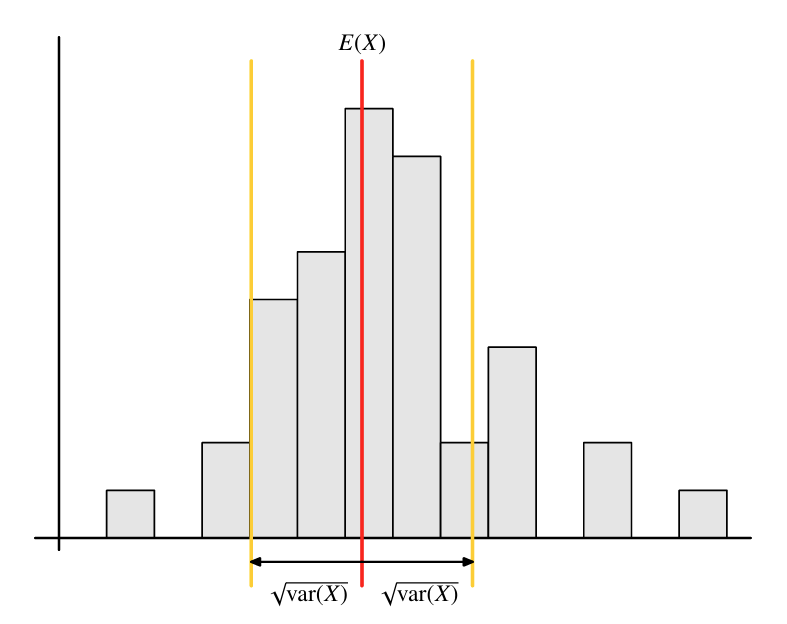
\includegraphics[width=1\linewidth]{Images/erwartungswert-varianz.png}
    \caption{Darstellung von Erwartungswert und Varianz}
    \label{fig:enter-label}
\end{figure}
\newpage
\section{Varianz}
Die \textbf{Varianz} (\href{https://de.wikipedia.org/wiki/Latein}{lateinisch} \textit{variantia} „Verschiedenheit“ bzw. \textit{variare} „(ver)ändern, verschieden sein“) ist ein \href{https://de.wikipedia.org/wiki/Streuungsma\%C3\%9F_(Statistik)}{Maß für die Streuung} einer Wahrscheinlichkeitsdichte um ihren Schwerpunkt. Mathematisch wird sie definiert als die \href{https://de.wikipedia.org/wiki/Mittlere_quadratische_Abweichung}{mittlere quadratische Abweichung} einer reellen \href{https://de.wikipedia.org/wiki/Zufallsvariable}{Zufallsvariablen} von ihrem \href{https://de.wikipedia.org/wiki/Erwartungswert}{Erwartungswert}. Sie ist das \href{https://de.wikipedia.org/wiki/Moment_(Stochastik)\#Zentrale_Momente}{zentrale Moment zweiter Ordnung} einer Zufallsvariablen. 

\defn{Varianz}{
Sei \(X: \Omega \rightarrow \mathbb{R}\)  eine Zufallsvariable, dann heisst die durch \(var(X)^2 = E((X-E(X))^2) \) definierte Grösse var(X) die Varianz von X. Oder auch die mittlere quadratische Abweichung vom Erwartungswert. Es ist insbesondere
\begin{equation}
    var(X) = E((X-E(X))^2) = E(X^2) - E(X)^2
\end{equation}

Man beachte, dass \(var(X)\) die Masseinheit des Quadrates von \(X\) hat. Wenn also \(X\) als Masseinheit eine Länge hat, dann hat \(var(X) \) die Masseinheit einer Fläche. Insbesondere kann man \(var(X)\) nicht in der gleichen Zeichnung visualisieren wie \(E(X)\). Aber die Grösse \(\sqrt{var(X)}\) hat die gleiche Masseinheit, sie drückt die “Streubreite” der Werte von \(X\).
}

\defn{Rechenregeln}{
Seien \(X\) und \(Y\) unabhängige Zufallsvariable, dann haben Summe und Produkt folgende Varianz
\begin{equation}
    \begin{split}
        var(\lambda X) &= \lambda^2 var(X) \\
        var(X+Y) &= var(X) + var(Y) \\
        var(XY) &= var(X) var(Y) + var(Y)E(X)^2 + var(X) E(Y)^2
    \end{split}
\end{equation}
}
\newpage

\section{Bewertung vom Mittelwert / Erwartungswert}
\defn{Tschebyscheff Ungleichung}{
\(X\) eine Zufallsvariable mit Erwartungswert \(\mu = E(X)\), dann lässt sich die Wahrscheinlichkeit, dass \(X\) um mehr als \(\epsilon\) vom Erwartungswert abweicht, wie folgt abschätzen: 
\begin{equation}
    P(|X- \mu| > \varepsilon) \leq \frac{var(x)}{\varepsilon^2}
\end{equation}
Lässt man \(\varepsilon\) wachsen findet man, dass Abweichungen deutlich grösser als \(\sqrt{var(X)}\) unwahrscheinlich sind.  
Leider sind die Vorhersagen wie auch bei der Tschebyscheff-Ungleichung nur beschränkt nützlich. Wenn die Wahrscheinlichkeit, dass der Mittelwert um mehr als \(\sigma\) vom Erwartungswert abweicht, kleiner als 1\% sein soll, sind dafür nach dem Gesetz der grossen Zahlen mindestens 100 Summanden nötig. 
}

\begin{figure}
    \centering
    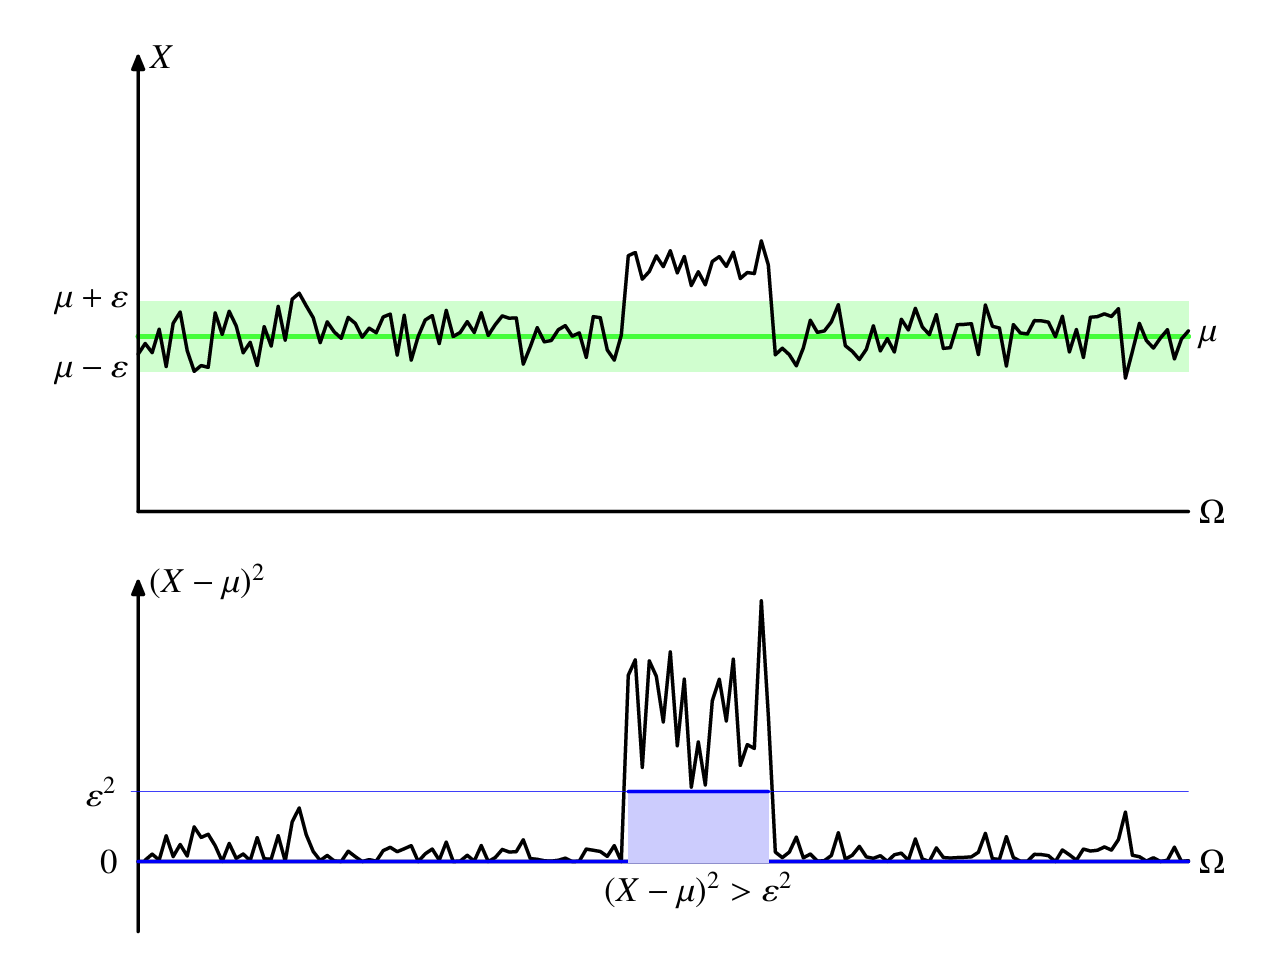
\includegraphics[width=0.75\linewidth]{Images/Tschebyscheff-Ungleichung.png}
    \caption{Herleitung der Tschebyscheff-Ungleichung, charakteristische Funktion des Er eignisses |X - µ| > \(\epsilon\) ist blau eingezeichnet. }
    \label{fig:enter-label}
\end{figure}

\newpage

\defn{Bernoulli Gesetz der grossen Zahlen}{
Die Wahrscheinlichkeit, dass der Mittelwert von \(n\) unabhängigen Zufallsvariablen mit Erwartungswert \(\mu\) und Varianz \(\sigma^2\) mehr als \(\varepsilon\) von \(\mu\) abweicht, ist :
\begin{equation}
    P(|M_n - \mu| > \varepsilon) \leq \frac{var(X)}{n\varepsilon^2}
\end{equation}
Insbesondere gilt
\begin{equation}
    \lim_{n \rightarrow \infty} P(|M_n - \mu| > \varepsilon) = 0
\end{equation}
}

\defn{Genauigkeit der empirischen Häufigkeit}{
Wird ein Experiment \(n\) mal durchgeführt, und tritt dabei das Ereignis \(A\) mit der relativen Häufigkeit \(h\)  ein, dann ist die Wahrscheinlichkeit, dass \(h\) um mehr als  \( \varepsilon\) von \(P(A)\) abweicht
\begin{equation}
    P(|h-P(A)| > \varepsilon ) \leq  \frac{P(A)(1-P(A))}{n \varepsilon^2} \leq \frac{1}{4n \varepsilon^2}
\end{equation}
}

\section{Lineare Regression}


\section{Verteil- und Dichtefunktionen}

\defn{Verteilfunktion}{
Die Verteilungsfunktion beschreibt die Wahrscheinlichkeiten der Werte einer Zufallsvariable:
\begin{equation}
    F(x)=P(X\leq x)
\end{equation}
}
\begin{figure}[H]
    \centering
    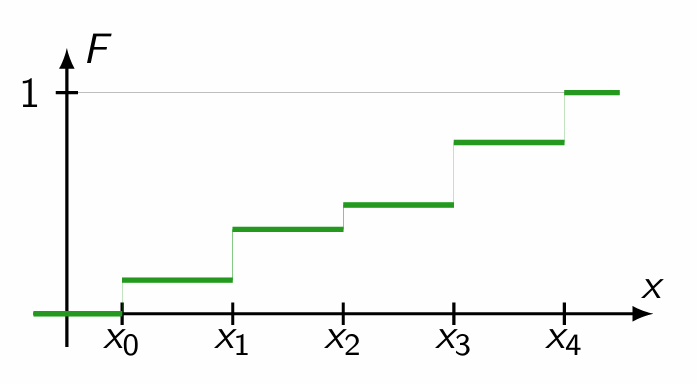
\includegraphics[width=0.5\linewidth]{Images/stetigef.png}
    \caption{Diskrete Verteilfunktion}
    \label{fig:enter-label}
\end{figure}
\begin{figure}[H]
    \centering
    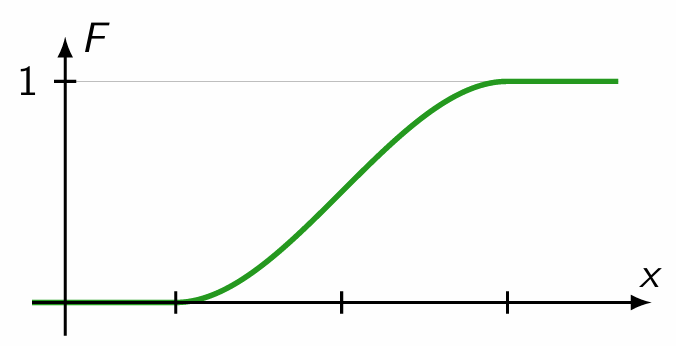
\includegraphics[width=0.5\linewidth]{Images/stetf.png}
    \caption{Stetige Verteilfunktion}
    \label{fig:enter-label}
\end{figure}
\begin{figure}[H]
    \centering
    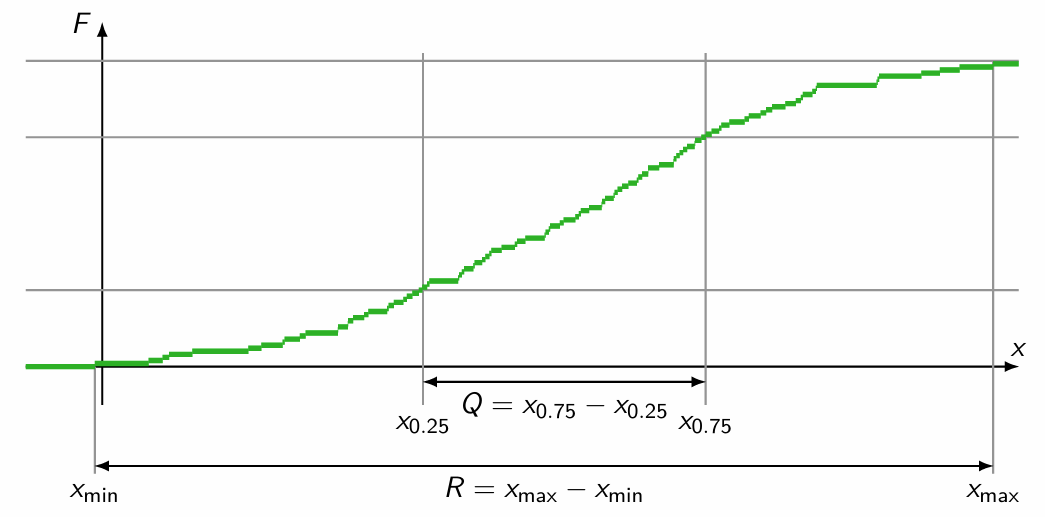
\includegraphics[width=1\linewidth]{Images/spannweitequartilabstand.png}
    \caption{Spannweite R und Quartilabstand Q}
    \label{fig:enter-label}
\end{figure}
%TBD definition Median
%Modus / Modalwert
%Mittelwert
%Gewichteter Mittelwert
%\subsection{Riemann- und Stieltjes-Integral}
\subsection{Wahrscheinlichkeitsdichte}
\begin{figure}[H]
    \centering
    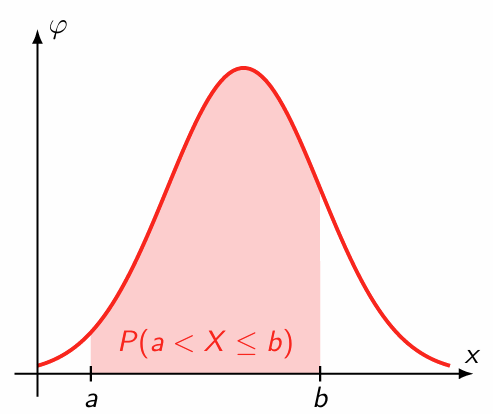
\includegraphics[width=0.5\linewidth]{Images/wahrscheinlichkeitsdichte.png}
    \caption{Wahrscheinlichkeitsdichte}
    \label{fig:enter-label}
\end{figure}
\defn{Wahrscheinlichkeitsdichte Funktion}{
Die Ableitung der Verteilungsfunktion heisst Wahrscheinlichkeitsdichte:
\begin{equation}
    \varphi(x)=\frac{d}{dx}F(x)=F'(X)
\end{equation}
Wenn \(F(x)\) (Verteilfunktion) die Stammfunktion ist bedeutet dies:
\begin{equation}
    P(a < X \leq b) = \int_a^b \varphi(x) dx
\end{equation}
Mit \(\varphi(x)\) kann man nun auch \(E(X)\) berechnen:
\begin{equation}
    \begin{split}
        E(X)&=\sum x \cdot p(x) \\
       & = \int_{-\infty}^\infty x \cdot \varphi(x)dx
    \end{split}
\end{equation}
}
%FALTUNG
\subsection{Gleichverteilung kreieren}
Durch erneute Anwendung der Verteilfunktion auf \(X\) wird die Zufallsvariable gleichverteilt.
\begin{figure}[H]
    \centering
    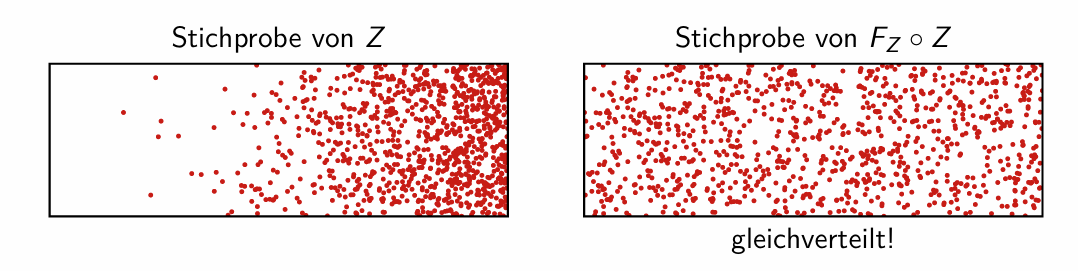
\includegraphics[width=0.75\linewidth]{Images/f_zaufz.png}
    \caption{Enter Caption}
    \label{fig:enter-label}
\end{figure}
\newpage
\section{Gleichverteilung}
\begin{figure}[H]
    \centering
    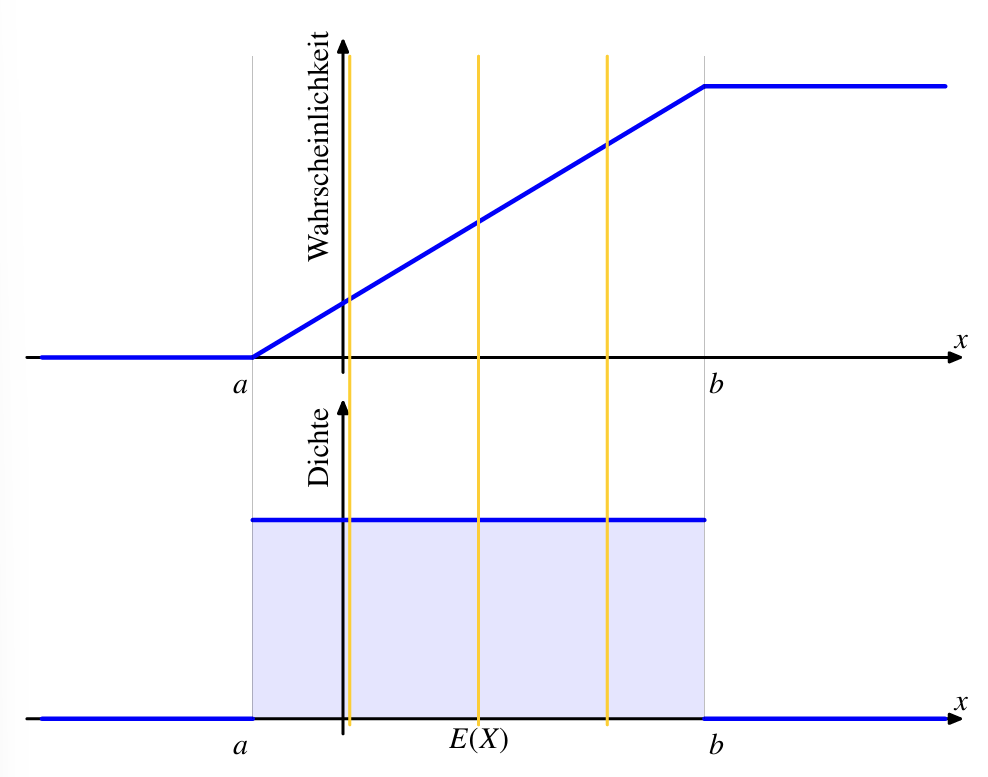
\includegraphics[width=1\linewidth]{Images/gleichverteilung.png}
    \caption{Gleichverteilung}
    \label{fig:enter-label}
\end{figure}
\defn{Dichtefunktion }{
\begin{equation}
    \varphi(x)=
    \begin{cases}
        \frac{1}{b-a} &a \leq x \leq b \\
        0 &\text{sonst}
    \end{cases}
\end{equation}
}
\defn{Verteilfunktion}{
    \begin{equation}
        F(x) = 
        \begin{cases}
            0  &x \leq a \\
            \frac{x-a}{b-a} &x \leq a \leq b \\
            1 &x > b
        \end{cases}
    \end{equation}
}
\defn{Erwartungswert}{
\begin{equation}
        E(X) = \frac{a+b}{2}
\end{equation}
}
\defn{Varianz}{
    \begin{equation}
        \sigma^2 = \frac{(b-a)^2}{12}
    \end{equation}
}
\defn{Median}{
\begin{equation}
    x_{\frac{1}{2}}=\frac{a+b}{2}
\end{equation}
}
\defn{Wahrscheinlichkeit für Abweichung}{
    \begin{equation}
        P(|X-E(X)|>\epsilon)=1\frac{2\epsilon}{b-a} \text{ für } \epsilon < \frac{b-a}{2}
    \end{equation}
}
\newpage

\end{document}

